%!TEX root = ../thesis.tex

\section{深層学習}

  深層学習(Deep learning)は,画像や音声などの複雑なデータを処理するための機械学習手法であり,人工ニューラルネットワークを基盤としている.\figref{Fig:deep_neural_network}に示すように,多層のニューロンが組み合わさり,人間の脳のような階層的な構造をしている.これにより,例えば画像や音声の特徴を学習し,自動的に認識や分類を行うことが可能になる.

  \begin{figure}[h]
    \centering
    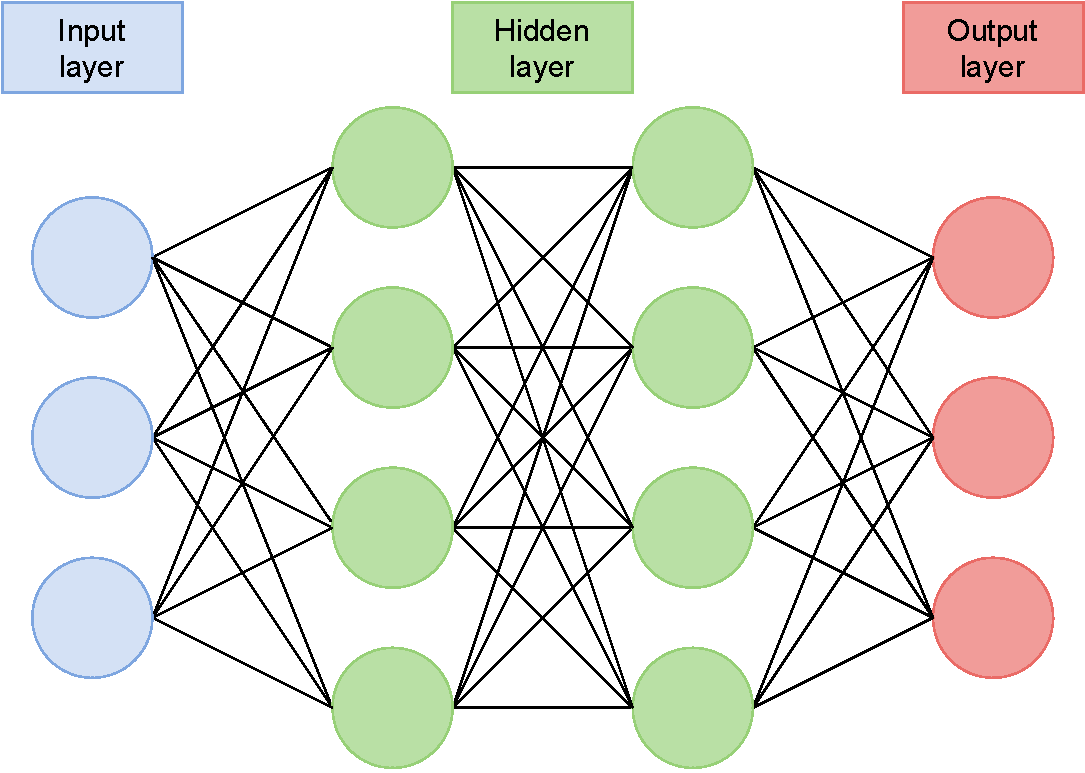
\includegraphics[keepaspectratio, scale=0.45] {images/pdf/deep_neural_network}
    \caption{Neural network}
    \label{Fig:deep_neural_network}
  \end{figure}

\newpage

\subsection{end-to-end学習}

  end-to-end学習は,\figref{Fig:Structure of general machine learning}に示すような一般的な機械学習の構造とは異なり,\figref{Fig:about_end-to-end}に示すような,システムの入力から出力までの全体の処理を一つのニューラルネットワークで直接学習する機械学習手法である.この手法では,画像や音声などの特徴抽出や前処理の段階を人手で設計する必要がなく,データから直接目標のタスクを学習することができる.

  \vspace{0.5cm}

  \begin{figure}[h]
    \centering
    \includegraphics[keepaspectratio, scale=0.80] {images/pdf/RobotGuidance_about_general_structure}
    \caption{Structure of general machine learning}
    \label{Fig:Structure of general machine learning}
  \end{figure}

  \begin{figure}[h]
    \centering
    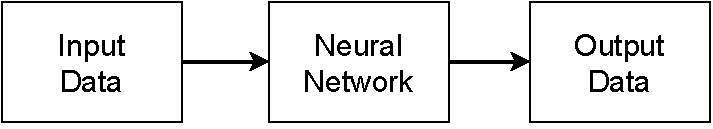
\includegraphics[keepaspectratio, scale=0.80] {images/pdf/RobotGuidance_about_end-to-end}
    \caption{Structure of end-to-end learning}
    \label{Fig:about_end-to-end}
  \end{figure}

\subsection{ミニバッチ学習}

  ミニバッチ学習は,データをミニバッチという小さなグループに分割してモデルを学習するアプローチである.通常,データセット全体を一度に処理するバッチ学習と,一つずつのデータを処理するオンライン学習の中間に位置する.

  \vspace{1cm}

  本研究は,オンライン(タスクを行いながらデータを収集)で学習(end-to-end学習とミニバッチ学習を組み合わせた学習)を行う.

\newpage

\subsection{Convolutional Neural Network (CNN)}

  本研究の学習器は畳み込みニューラルネットワーク(Convolutional Neural Network:CNN)で,これは画像認識などで用いられている\cite{yann1}\cite{alex}.畳み込み層とプーリング層を含む構造で,多次元配列の形式データを効率的に処理するように設計されている.例として,LeCunら\cite{yann1}は,畳み込み層とプーリング層を連続して接続するネットワークを用いることで,手書き文字を識別できることを示した(\figref{Fig:yann_CNN}).また,Krizhevskyら\cite{alex}は,深い畳み込みニューラルネットワークを用いることで,1000種類のクラスに分類できることを示し(\figref{Fig:deep_convolutional_neural_networks}),ILSVRC(ImageNet Large Scale Visual Recognition Challenge)2012で優勝した.

  CNNは,主に畳み込み層,プーリング層,および全結合層から構成される.以下に,それぞれの特徴を記す.

  \begin{enumerate}
    \item 畳み込み層\\
    入力データに対してフィルターを適用し,特徴を抽出した特徴マップを出力する層
    \item プーリング層\\
    特徴マップのサイズを削減し,特徴の位置に対する頑健性を向上させるために,領域内の最大値や平均値を取る操作を行う層
    \item 全結合層\\
    畳み込み層とプーリング層で抽出された特徴を組み合わせて,最終的な出力を生成する層
  \end{enumerate}

  \begin{figure}[h]
    \centering
    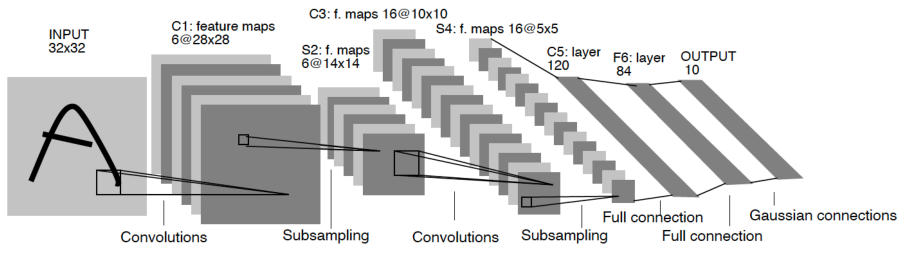
\includegraphics[keepaspectratio, scale=0.80] {images/pdf/yann_CNN}
    \caption[Training the neural network]{Training the neural network (source: \cite{yann1})}
    \label{Fig:yann_CNN}
  \end{figure}

\newpage

  \begin{figure}[h]
    \centering
    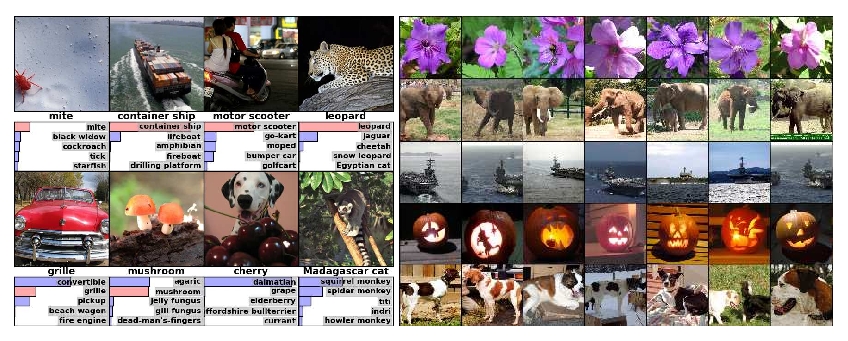
\includegraphics[keepaspectratio, scale=0.80] {images/pdf/deep_convolutional_neural_networks}
    \caption[ImageNet classification with deep convolutional neural network]{ImageNet classification with deep convolutional neural network (source: \cite{alex})}
    \label{Fig:deep_convolutional_neural_networks}
  \end{figure}


\newpage

